% SPDX-License-Identifier: CC-BY-4.0
%
% Copyright (c) 2023 Nelson Vieira
%
% @author Nelson Vieira <2080511@student.uma.pt>
% @contributor Mary Barreto <mary.barreto@staff.uma.pt>
% @license CC-BY-4.0 <https://creativecommons.org/licenses/by/4.0/legalcode.txt>
\section{Methodology} \label{section:methodology}

The overall work is comprised of two phases which will be described
in the following paragraphs. The first phase, which is primarily described
on Chapter \ref{section:state_of_the_art}, focuses on gathering the state
of the art in terms of the most relevant topics, from which the main privacy
concepts were selected to be explored in the first stage of phase two with
the creation of a questionnaire with the aim to collect user perceptions
of privacy. The second stage of phase 2 consisted in developing an
application, partially based on the information generated by the survey,
that can identify what sort of devices are around, what kind of data is
gathered by these devices, present privacy options to the user when available,
and what can be done to prevent undesirable data from being collected.
\par
The first phase involved conducting a systematic literature review to gather
the most relevant papers discussing methodologies and techniques for the
protection of user privacy data with a focus on IoT systems. This SLR focused
on papers from the last 13 years, from 2010 until 2023, since papers
published prior to 2010 become out of date with the evolution of technology.
Although certain aspects of privacy have remained constant throughout the years,
this historical perspective on privacy is primarily discussed in the
introduction to this work.

The SLR followed Keshav's three-pass approach \cite{KeshavHow} and
PRISMA 2020 \cite{pagen2021prisma} guidelines when selecting the papers
for review, the principles suggested by Kitchenham and Charters \cite{kitchenham2007guidelines}
were also taken into account in order to ensure the transparency and
reliability of the review. On Keshav's approach, first the title would
be read, then the abstract, the introduction and conclusion and briefly
skim the rest of the paper and then decide if it was worth reading any
further. If the document passed the inclusion criteria, which will be
discussed further ahead, then the document would be read in its entirety
while ignoring any tables, figures, images or graphs. If the paper failed
to present any interesting idea, approach, or technique it would be discarded,
but if not, it would be read carefully from the beginning again in order
to fully understand what it presents.
% Figure \ref{} represents this process.

It is challenging to curate the literature and
gain an in-depth understanding of its different aspects due to the vast
array of approaches that address the topic IoT privacy. As a result, specific
databases were used because of the sheer quantity of papers contained within
them makes research easier. The following were the primary databases of the SLR:

\begin{itemize}
    \item[$\bullet$]
    Google Scholar;
    \item[$\bullet$]
    ScienceDirect;
    \item[$\bullet$]
    IEEE Explore Digital Library;
    \item[$\bullet$]
    ResearchGate;
    \item[$\bullet$]
    Elicit;
    \item[$\bullet$]
    BASE.
\end{itemize}

Other supplementary databases used, during the course of the research, include
CORE, AIS, ACM Digital Library, Semantic Scholar, Baidu Scholar, RefSeek and
Science.gov. These databases were used in to search certain works that
would have not been found otherwise.

The papers were collected by searching the databases with keywords, a broad
spectrum of results were obtained using generic terms like. The primary search
terms were used between quotation marks, e.g., ``Internet of Things'', so that
results include all words in sequence, operators AND and OR were also used
as was a minus sign before a keyword to remove said keyword from the search
results. Many search terms were utilized, however the most often
used ones, based on their frequency, include: ``Digital literacy'',
``Differential privacy'', ``Privacy paradox'', ``Machine learning'',
``Blockchain'', ``User awareness'', ``User knowledge'', ``Blockchain'',
``Privacy concerns'', ``Privacy perceptions'', ``Regulation'',
``Framework'', ``Security'', ``Deep learning'', ``Approach''.
Most of these search terms also included the terms ``Privacy'' and/or
``Internet of Things'' or any variants like ``IoT'' or ``IoT privacy''.

The SLR attempts to summarize and evaluate IoT privacy concerns, as well
as ideas, techniques, or methodologies to overcome those challenges.
The focal point in this phase was answering the following question: Does
the paper present a new methodology or interesting angle to tackle users'
privacy concerns?
% A better restatement of inclusion criteria is formulated
% in the following research questions:\\

% \vspace{5mm}
% \textbf{Phase 1 (Literature review):} \\

% \textbf{RQ1:} What approaches are currently being considered to address privacy
% issues in IoT?

% \textbf{RQ2:} What issues are prevalent in IoT that make it challenging to
% protect individuals privacy? \\

As referenced before, only papers published from 2010 until 2023 are considered,
these works must also be published in journals, conference proceedings, dissertations,
thesis or technical reports. Exclusion criteria include presentations, editorials,
abstracts or commentaries. Works can cover any area as long as they deal with
privacy in the Internet of Things, if the paper does not cover IoT then at least
it must cover privacy aspects that can be applied to IoT, as is the case of the
privacy paradox.

From database searches, a total of 229 papers were found. Applying the inclusion
and exclusion criteria to these papers bring the total number of papers down to
95, excluding 134 papers. After reading the full texts of the remaining 95 papers,
47 were excluded, making the number of total papers in the SRL be 48.

Having collected the major findings of the SLR, this work then aimed to conduct a
throughout study split into two stages, which will compose phase 2 of this work.
% The following research questions will be made for this phase:\\

% \vspace{5mm}
% \textbf{Phase 2 (Survey and application):} \\

% \textbf{RQ3:} What are the perceptions of individuals on online privacy?

% \textbf{RQ4:} How can users be empowered to protect their privacy in IoT systems?\\
% \vspace{5mm}

The second phase was evaluated on two stages, the first one consisted
in doing a questionnaire on people's general privacy concerns, while using and interacting
with IoT devices. The SLR helped on the creation of the questionnaire to
assess general user's knowledge on privacy concepts, their habits and concerns,
their understanding of privacy rights, and what they do to safeguard those
rights. The goal of this study was to both understand the privacy paradox
and collect insights on how to address privacy issues in IoT devices.

% Having collected the major findings, this work then aims to conduct a throughout
% study split in several stages and around the following research questions:

% \textbf{RQ1:} What approaches are being considered for privacy issues in
% IoT in the currently available literature?

% \textbf{RQ2:} What IoT-related tools are available that empower users to
% protect their privacy rights? OR How to empower users to protect their privacy
% rights?

% \textbf{RQ3:} What issues are prevalent in IoT that make it difficult to
% address privacy and security problems?

% The proposed methodology is composed of two phases, the first phase consists
% on doing a study on people's general privacy concerns while using and interacting
% with IoT devices. This study will consist on preparing a questionnaire to
% assess general user's knowledge on privacy concepts, their habits and concerns,
% their understanding of privacy rights, and what they do to safeguard those
% rights. The goal of this study is to both understand the privacy paradox
% and collect data on their proposal to address privacy issues with regard
% to IoT devices. The second phase consists in developing an application, partially
% based on the information generated by the survey, that can identify what sort
% of devices are around, what kind of data is gathered by these devices, present
% privacy options to the user where available, and what can be done to prevent
% undesirable data from being collected.

% The second phase consists
% in doing an application that can detect IoT devices nearby the user with.
% The application should do the following when
% detecting a device:
% 1. it should show some information about the device;
% 2. it should categorize the device;
% 3. it should provide the user with privacy options, if the device allows the
% user to decline data harvesting.
% This application at first sight might appear to be a mere privacy assistant
% but it is not, because IoT assistants merely choose what privacy options the
% user first sets and maintains it for every other application that the user
% might use. The proposed app does not have the objective to conform to the user's
% preferred privacy choices, it merely informs the user about nearby IoT devices
% and can provide the user with privacy options. But the main objective is creating
% awareness in individuals about the various devices that are around and make
% the user questions their choices.

\subsection{User perceptions}

This questionnaire aims to understand people's perception of IoT and their privacy
practices online. It also serves to better understand and demystify the privacy
paradox and to help provide a solution to the privacy issue in IoT, which will be
discussed on Chapter \ref{section:stage2}.

The questionnaire consisted of 86 questions divided into 7 sections to
gauge users' digital literacy, the first section being about general privacy
questions, then about the predisposition to data sharing, to concerns with
privacy then about daily digital routines, then about profile identification,
subsequently about IoT general knowledge before a final part about
non-identifiable demographic data. The questionnaire's structure is shown
in more detail in Table \ref{table:questionnaire}, the full questionnaire
is presented on \nameref{appendix:survey}.

\begin{table}[H]
    \begin{center}
        \begin{tabular}{r *{3}{ p{6cm} }}
            \hline
            \textbf{\#}\hspace{0.5cm} & \textbf{Section} & \textbf{Details} \\
            \hline
            1\hspace{0.5cm} & General knowledge and attitudes towards privacy & This
            section's goal is to ask generic questions regarding the participants awareness
            of information privacy. \\
            \hline
            2\hspace{0.5cm} & Disposition for sharing personal information & This
            section is designed to elicit generic inquiries about the participants
            willingness to provide personal information. \\
            \hline
            3\hspace{0.5cm} & Privacy concerns & This section strives to
            elicit questions about potential concerns about disclosing
            personal information. \\
            \hline
            4\hspace{0.5cm} & Current online habits and practices & This
            section includes general questions with regard to working with
            the internet in everyday activities. \\
            \hline
            5\hspace{0.5cm} & Profile identification & This section gathers
            more particular questions concerning employing profiles to make
            it more straightforward to generate tailor-made interactions. \\
            \hline
            6\hspace{0.5cm} & Knowledge and habits regarding the Internet
            of Things & This section contains questions about participants'
            usage patterns for IoT devices as well as questions that aim to
            understand their level of literacy. \\
            \hline
            7\hspace{0.5cm} & Demographic data & This section is for
            gathering broad demographic information that allows
            to characterize the participants in statistical terms. \\
            \hline
        \end{tabular}
    \end{center}
    \vspace{1em}
    \caption{Structure of the questionnaire.}
    \label{table:questionnaire}
\end{table}

Great care was taken when it comes to this questionnaire's data collection, in
order to not identify any individual or group of individuals, for
instance, when it comes to differential privacy, any data that might
identify someone will not be disclosed, even though the data might suffer
from some inaccuracy because of this.

The scale that was used in the questionnaire, which is from one to seven,
is based on the work of Philip K. Masur \cite{masur2018situational}, it
was chosen because it provides a more nuanced understanding
of the knowledge of participants. This scale was developed as an
online privacy concerns scale so it fits perfectly on this questionnaire,
another scale, also developed by Masur with Teutsch and Trepte,
that could be used but was ultimately not chosen is the Online Privacy
Literacy Scale \cite{masur2017entwicklung}, although the questionnaire does
contain some of the main aspects of this scale like knowledge of data collection and
analysis practices by institutions and online service providers
knowledge of data protection law, knowledge of technical aspects of data
protection and knowledge of data protection strategies.
This survey was partially based in a study done in the Philippines by the
government in the context of their privacy act of 2012 \cite{Philippine2022Conduct},
this was the second survey done on the country's population. It was also
inspired by Alves's master thesis \cite{alves2021}, which was about citizen's
perception about privacy in the wake of GDPR.

This survey was constructed in Google Forms and distributed through the internet,
the intent would be that this would reach as many individuals as possible,
besides Google Forms itself, it was used other online venues for distribution
like social media, forum websites, through in person discussions and
some participants responded when also doing the application usability tests.

The questionnaire was available for completion until August 30, 2023,
and during the time that it was open 45 participants responded.
Several online survey dissemination services were used to acquire participants,
all the services used were based on the goodwill of the participants, there
was no financial incentive for completing the survey. Most of the services
used were software as a service (SaaS), these platforms are based
on credits for filling in other questionnaires available, this makes the process
of acquiring participants very tedious as many questionnaires need to be
filled in to get a reasonable number of participants, which ideally would be
at least around 150 to 200 participants. Disseminating the questionnaire in this way does not
entail any additional cost, but it may mean that the results obtained
may not be as accurate as they could have been, as some participants may
be completing this questionnaire quickly just to get the number of participants
for their own questionnaires, although there is no way to guarantee that
participants would answer the questionnaire as genuinely as possible if there
was some sort of financial incentive. In addition to
dissemination by the various services, social networks were also used as well
as it was personally disseminated to relatives and close acquaintances.
An in-person dissemination strategy could have been used, it was not adopted
because it would be a very sluggish approach to obtain responses,
additionally, people could have felt compelled to respond haphazardly.

From the respondents, 47\% are male and 51\% are female, while 2\% do not identify
as neither, see Figure \ref{fig:genre}. 40\% of the participants are younger
than 25 years old, 31.11\% are aged between 26 and 35, 9\% are between
36 and 45 years old, 18\% are older than 46 but younger than 65 and 2\%
have more than 65 years, as shown in Figure \ref{fig:age}.

\begin{figure}[H]
    \begin{center}
        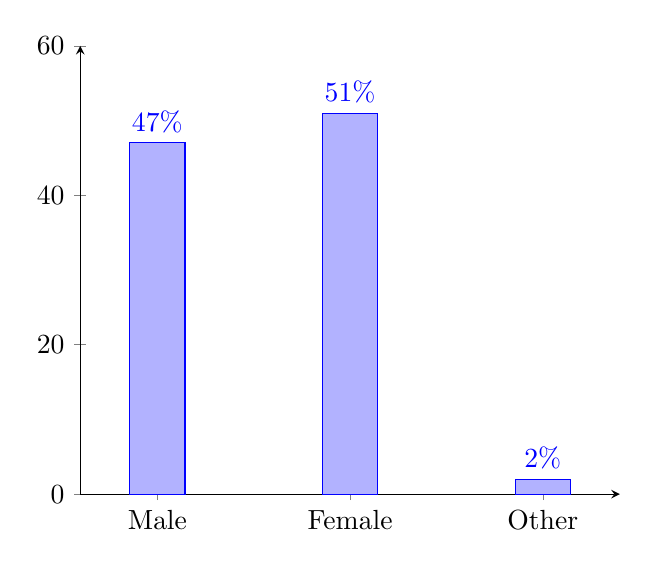
\begin{tikzpicture}
            \begin{axis}[
                ybar,
                bar width=20pt,
                ymin=0,
                ymax=60,
                symbolic x coords={Male,Female,Other},
                xtick=data,
                axis x line=bottom,
                axis y line=left,
                enlarge x limits=0.2,
                nodes near coords={\pgfmathprintnumber\pgfplotspointmeta\%}
            ]
                \addplot coordinates {(Male,47) (Female,51) (Other,2)};
            \end{axis}
        \end{tikzpicture}
        \caption{Genre distribution of participants.}
        \label{fig:genre}
    \end{center}
\end{figure}

\begin{figure}[H]
    \begin{center}
        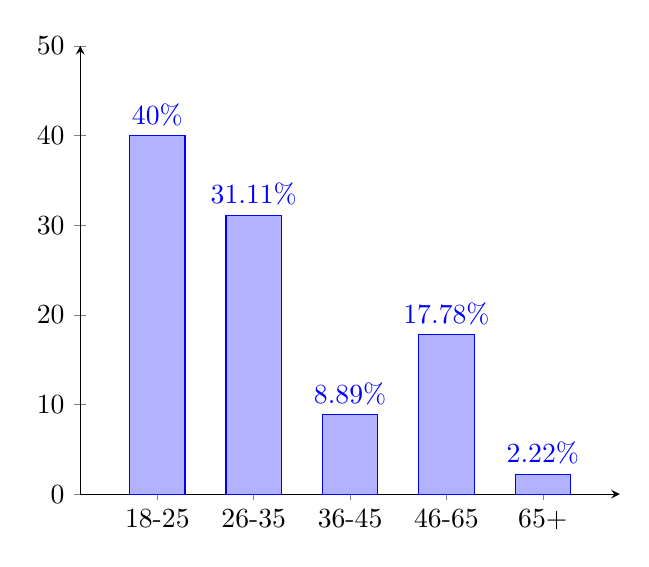
\begin{tikzpicture}
            \begin{axis}[
                ybar,
                bar width=20pt,
                ymin=0,
                ymax=50,
                symbolic x coords={18-25,26-35,36-45,46-65,65+},
                xtick=data,
                axis x line=bottom,
                axis y line=left,
                enlarge x limits=0.2,
                nodes near coords={\pgfmathprintnumber\pgfplotspointmeta\%}
            ]
                \addplot coordinates {(18-25,40) (26-35,31.11) (36-45,8.89) (46-65,17.78) (65+,2.22)};
            \end{axis}
        \end{tikzpicture}
        \caption{Age ranges of participants.}
        \label{fig:age}
    \end{center}
\end{figure}

Most of the respondents have a bachelor's degree, 66.67\% to be exact, 17.78\% have
only finished high school, 2.22\% only have a basic education, 11.11\%
have a master's degree and 2.22\% have a doctorate, as pictured in Figure \ref{fig:education}.

\begin{figure}[H]
    \begin{center}
        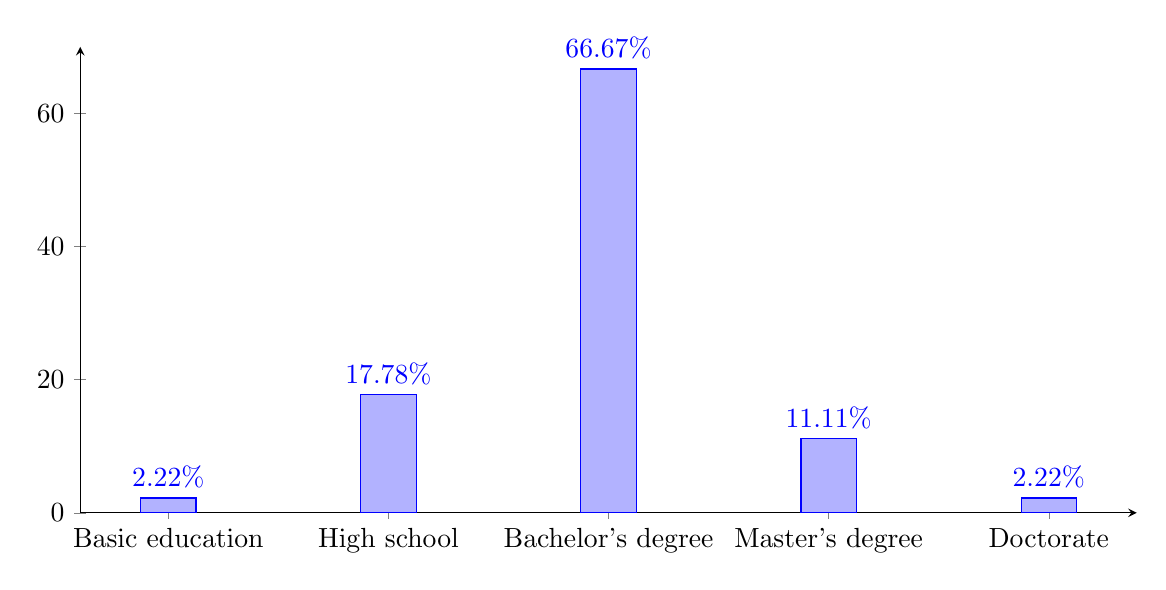
\begin{tikzpicture}
            \begin{axis}[
                height=7.5cm,
                width=15cm,
                ybar,
                bar width=20pt,
                ymin=0,
                ymax=70,
                symbolic x coords={Basic education,High school,Bachelor's degree,Master's degree,Doctorate},
                xtick=data,
                axis x line=bottom,
                axis y line=left,
                enlarge x limits=0.1,
                nodes near coords={\pgfmathprintnumber\pgfplotspointmeta\%}
            ]
                \addplot coordinates {(Basic education,2.22) (High school,17.78) (Bachelor's degree,66.67) (Master's degree,11.11) (Doctorate,2.22)};
            \end{axis}
        \end{tikzpicture}
        \caption{Education qualifications distribution of participants.}
        \label{fig:education}
    \end{center}
\end{figure}

Most survey participants, 60\%, are from Portugal, 20\% are from the USA,
4.44\% from the UK while 15.66\% are divided between the following countries:
Germany, Australia, Sweden, Netherlands, China, Indonesia and Canada as shown
in Figure \ref{fig:country}.

\begin{figure}[H]
    \begin{center}
        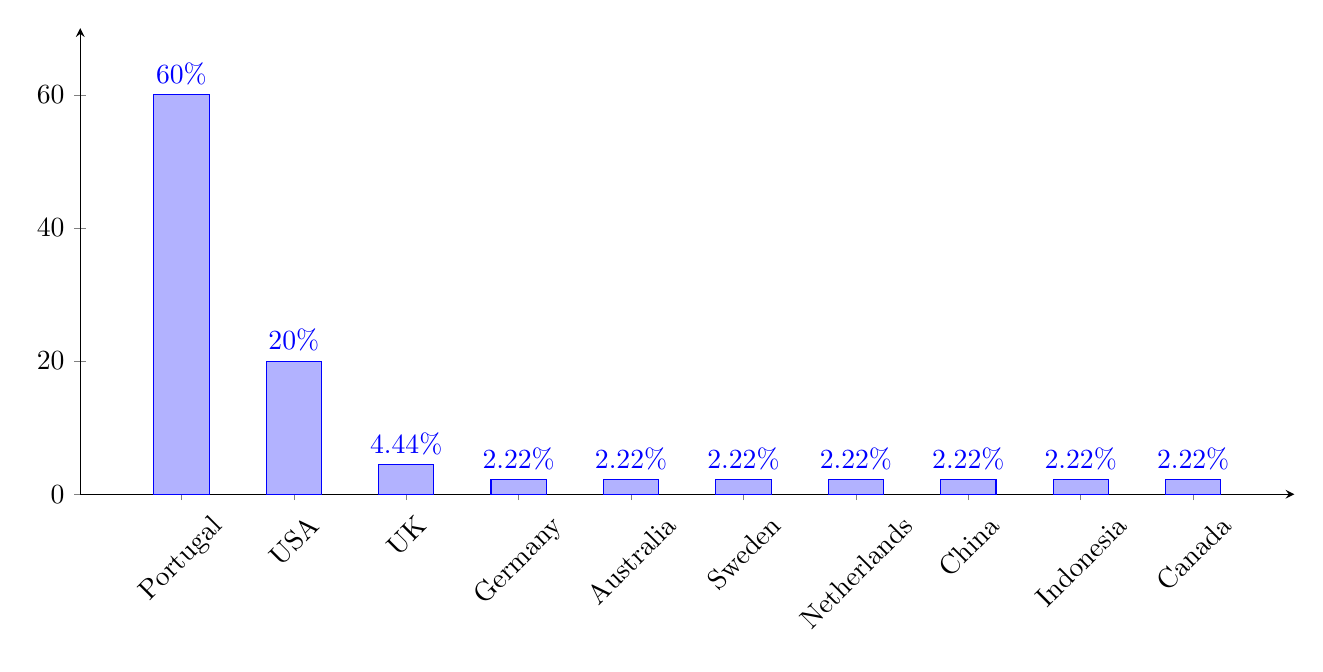
\begin{tikzpicture}
            \begin{axis}[
                height=7.5cm,
                width=17cm,
                ybar,
                bar width=20pt,
                ymin=0,
                ymax=70,
                symbolic x coords={Portugal,USA,UK,Germany,Australia,Sweden,Netherlands,China,Indonesia,Canada},
                xtick=data,
                xticklabel style={rotate=45},
                axis x line=bottom,
                axis y line=left,
                enlarge x limits=0.1,
                nodes near coords={\pgfmathprintnumber\pgfplotspointmeta\%}
            ]
                \addplot coordinates {(Portugal,60) (USA,20) (UK,4.44) (Germany,2.22) (Australia,2.22) (Sweden,2.22) (Netherlands,2.22) (China,2.22) (Indonesia,2.22) (Canada,2.22)};
            \end{axis}
        \end{tikzpicture}
        \caption{Distribution of participants by country of residence.}
        \label{fig:country}
    \end{center}
\end{figure}

Figure \ref{fig:annual_income} depicts the annual income, by range, of participants. 35.56\%
of participants get an annual income below 10 000\textup{\euro} while 17.78\% received
between 10 000\textup{\euro} and 20 000\textup{\euro}, 17.78\% between 20 000\textup{\euro}
and 50 000\textup{\euro}, 6.67\% 50 000\textup{\euro} and 100 000\textup{\euro},
and 22.22\% of participants preferred not to disclose.

\begin{figure}[H]
    \begin{center}
        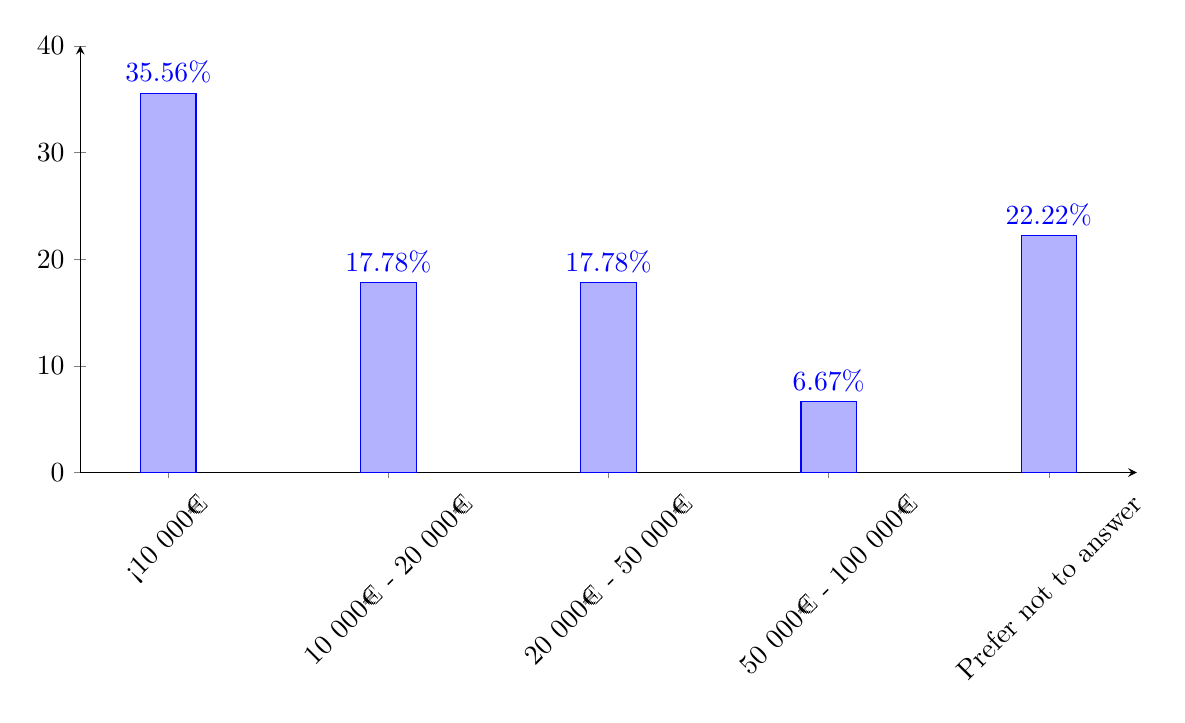
\begin{tikzpicture}
            \begin{axis}[
                height=7cm,
                width=15cm,
                ybar,
                bar width=20pt,
                ymin=0,
                ymax=40,
                symbolic x coords={<10 000€,10 000€ - 20 000€,20 000€ - 50 000€,50 000€ - 100 000€,Prefer not to answer},
                xtick=data,
                xticklabel style={rotate=45},
                axis x line=bottom,
                axis y line=left,
                enlarge x limits=0.1,
                nodes near coords={\pgfmathprintnumber\pgfplotspointmeta\%}
            ]
                \addplot coordinates {(<10 000€,35.56) (10 000€ - 20 000€,17.78) (20 000€ - 50 000€,17.78) (50 000€ - 100 000€,6.67) (Prefer not to answer,22.22)};
            \end{axis}
        \end{tikzpicture}
        \caption{Distribution of participants per annual income.}
        \label{fig:annual_income}
    \end{center}
\end{figure}
